\documentclass[a4paper,landscape]{scrartcl}
\usepackage{fancybox}
\usepackage{tikz}
\usepackage{listings,lstautogobble}
\usepackage[makeroom]{cancel}
\pagenumbering{gobble}
\renewcommand\CancelColor{\color{red}}
\usepackage{xcolor}
\usepackage{color}
\usepackage{eso-pic}
\definecolor{RoyalBlue}{cmyk}{1, 0.50, 0, 0}
\lstset{escapeinside={<@}{@>}}

\lstset{language=SQL,
keywordstyle=\color{RoyalBlue},
basicstyle=\scriptsize\ttfamily,
commentstyle=\ttfamily\itshape\color{gray},
stringstyle=\ttfamily,
showstringspaces=false,
breaklines=true,
frameround=ffff,
frame=single,
rulecolor=\color{black},
autogobble=true
}
\tikzstyle{red state}=[
draw = red,
thick,
fill = white,
minimum size = 4mm,
circle
]

%\title{MergeSort-RecursionTree}
%\author{Manuel Kirsch}
%\date{}
\begin{document}
%    \ovalbox{
%    \begin{center}
    \begin{figure}
        \centering
        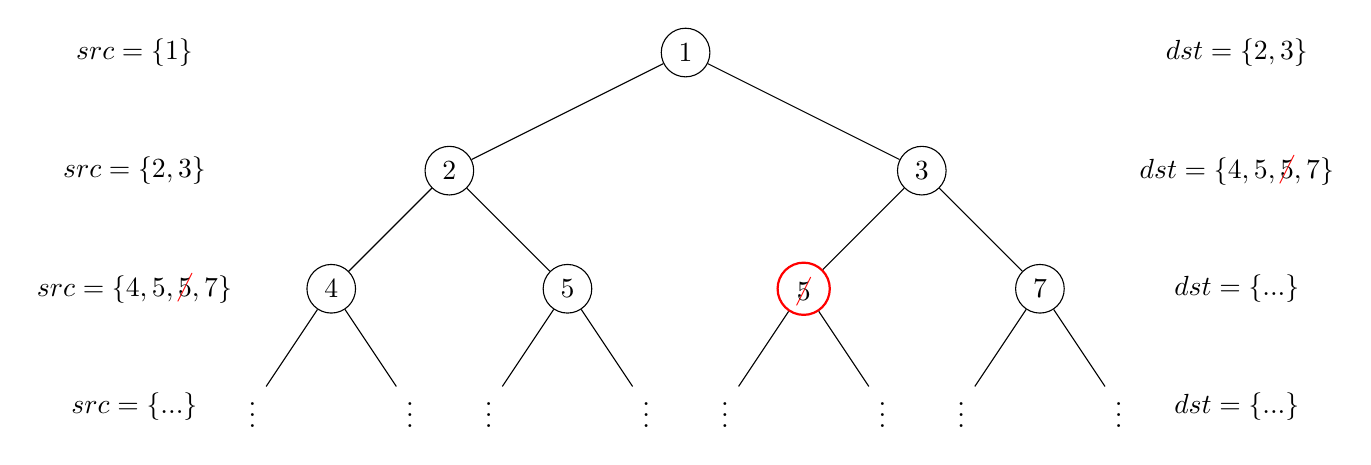
\begin{tikzpicture}[level/.style={sibling distance=60mm/#1}]
            \node [circle,draw] (z){$1$}
            child {node [circle,draw] (a) {$2$}
            child {node [circle,draw] (b) {$4$}
            child {node {$\vdots$}
            child [grow=left] {node (q) {$src = \{...\}$} edge from parent[draw=none]
            child [grow=up] {node (q) {$src = \{4,5,\cancel{5},7\}$} edge from parent[draw=none]
            child [grow=up] {node (q) {$src = \{2,3\}$} edge from parent[draw=none]
            child [grow=up] {node (q) {$src = \{1\}$} edge from parent[draw=none]}
            }
            }
            }
            }
            child {node {$\vdots$}}
            }
            child {node [circle,draw] (b) {$5$}
            child {node {$\vdots$}}
            child {node {$\vdots$}}
            }
            }
            child {node [circle,draw] (j) {$3$}
            child {node [red state] (k) {$\cancel{5}$}
            child {node {$\vdots$}}
            child {node {$\vdots$}}
            }
            child {node [circle,draw] (l) {$7$}
            child {node {$\vdots$}}
            child {node {$\vdots$}
            child [grow=right] {node (q) {$dst = \{...\}$} edge from parent[draw=none]
            child [grow=up] {node (q) {$dst = \{...\}$} edge from parent[draw=none]
            child [grow=up] {node (r) {$dst = \{4,5,\cancel{5},7\}$ } edge from parent[draw=none]
            child [grow=up] {node (u) {$dst = \{2,3\}$ } edge from parent[draw=none]}
            }
            }}}
            }
            };
        \end{tikzpicture}


        %}

        \begin{lstlisting}[language=SQL,caption = selectRecursive,frame=single]
            SELECT <@\textcolor{red}{DISTINCT(dst)}@> FROM team22.relation_facebook WHERE src IN(
                SELECT <@\textcolor{red}{DISTINCT(dst)}@> FROM team22.relation_facebook WHERE src IN(
                    SELECT <@\textcolor{red}{DISTINCT(dst)}@> FROM team22.relation_facebook WHERE src IN(1)
                )
            )
        \end{lstlisting}
        \begin{lstlisting}[language=SQL,caption = selectWithJoin,frame=single]
            SELECT <@\textcolor{red}{DISTINCT(rf3.dst)}@>
                FROM public.relation_facebook rf1,
                    public.relation_facebook rf2,
                    public.relation_facebook rf3
                WHERE rf2.src = rf1.dst
                    AND rf3.src = rf2.dst
                    AND rf1.src = 765;
        \end{lstlisting}

%    \end{figure}
%    \begin{figure}
    \end{figure}
    \newpage

        \begin{figure}
            \centering

            \begin{lstlisting}[language=SQL,caption = StoredProcedure,frame=single]
                CREATE OR REPLACE FUNCTION recursivesearch(tInput integer[], iRecursionDepth integer, sTable text) RETURNS SETOF integer AS $$
                    Declare
                    intermDst_ integer[];
                    iCount integer;
                    BEGIN
                    CREATE TABLE intermDst AS SELECT * FROM unnest(tInput);
                    EXECUTE 'CREATE TABLE intermDst1 AS SELECT DISTINCT(dst) FROM ' || sTable || ' WHERE src IN (SELECT * FROM intermDst)';
                    -- Does not return from function!
                    return query SELECT * FROM intermDst1;
                    -- Does not return from function!
                    intermDst_ := ARRAY(SELECT * FROM intermDst1);
                    raise notice 'timestamp: %', clock_timestamp();
                    SELECT count(*) INTO iCount FROM intermDst;
                    raise notice 'Count Table: %', iCount;
                    DROP TABLE intermDst;
                    DROP TABLE intermDst1;
                    if iRecursionDepth > 1 THEN
                    return query SELECT * FROM recursivesearch(intermDst_, iRecursionDepth - 1, sTable);
                    ELSE
                    RETURN;
                    END IF;
                    END;
                $$ LANGUAGE plpgsql;
            \end{lstlisting}

        \end{figure}
        \newpage
        \begin{figure}
        \centering
        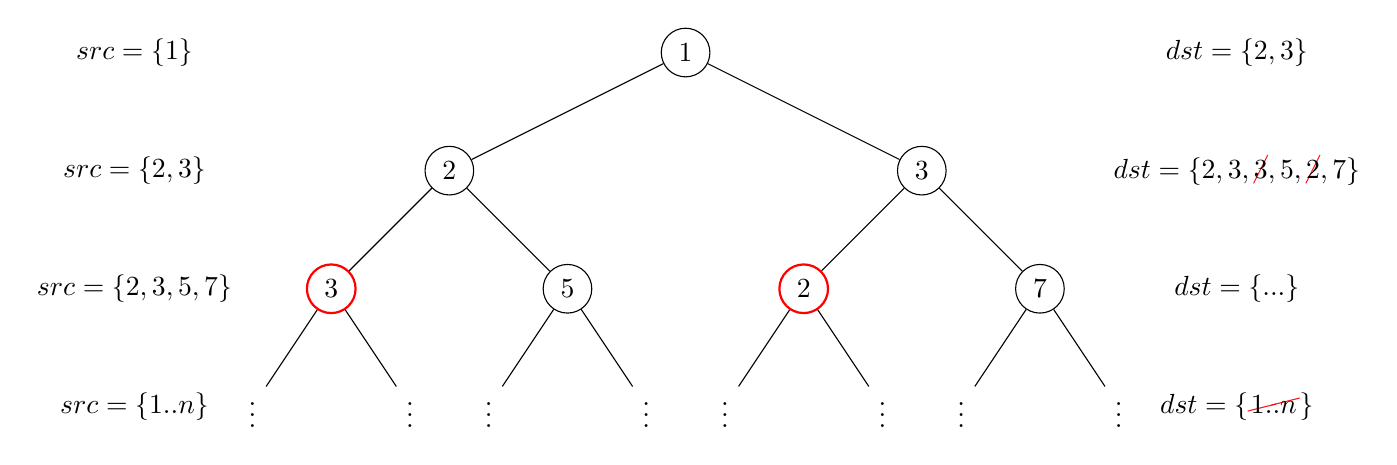
\begin{tikzpicture}[level/.style={sibling distance=60mm/#1}]
            \node [circle,draw] (z){$1$}
            child {node [circle,draw] (a) {$2$}
            child {node [red state] (b) {$3$}
            child {node {$\vdots$}
            child [grow=left] {node (q) {$src = \{1..n\}$} edge from parent[draw=none]
            child [grow=up] {node (q) {$src = \{2,3, 5,7\}$} edge from parent[draw=none]
            child [grow=up] {node (q) {$src = \{2,3\}$} edge from parent[draw=none]
            child [grow=up] {node (q) {$src = \{1\}$} edge from parent[draw=none]}
            }
            }
            }
            }
            child {node {$\vdots$}}
            }
            child {node [circle,draw] (b) {$5$}
            child {node {$\vdots$}}
            child {node {$\vdots$}}
            }
            }
            child {node [circle,draw] (j) {$3$}
            child {node [red state] (k) {$2$}
            child {node {$\vdots$}}
            child {node {$\vdots$}}
            }
            child {node [circle,draw] (l) {$7$}
            child {node {$\vdots$}}
            child {node {$\vdots$}
            child [grow=right] {node (q) {$dst = \{\cancel{1..n}\}$} edge from parent[draw=none]
            child [grow=up] {node (q) {$dst = \{...\}$} edge from parent[draw=none]
            child [grow=up] {node (r) {$dst = \{2,3, \cancel{3},5,\cancel{2},7\}$ } edge from parent[draw=none]
            child [grow=up] {node (u) {$dst = \{2,3\}$ } edge from parent[draw=none]}
            }
            }}}
            }
            };
        \end{tikzpicture}

            \begin{lstlisting}[language=SQL,caption = selectWithUnion,frame=single]
                WITH RECURSIVE graphtraverse AS(
                    SELECT DISTINCT(dst)
                        FROM
                            public.relation_facebook
                        WHERE
                            src =765
                    <@\textcolor{red}{UNION} @>
                    SELECT p.dst
                        FROM
                            relation_facebook p
                        WHERE
                            src IN ( p.src )
                    )
                SELECT * FROM graphtraverse
            \end{lstlisting}
        \end{figure}

%    \end{center}

\end{document}